\documentclass{article}
\usepackage{listings}
\usepackage{graphicx}
\usepackage{float}
\DeclareGraphicsExtensions{.jpeg,.png}

\graphicspath{ {/Users/llaryssa/Documents/Stevens/CS532-3DCV/CS532-assignments/assignment4/imgs/} }

\begin{document}

\centerline{\sc \large CS 532: Homework Assignment 4}
\vspace{.5pc}
\centerline{Alana Laryssa Seabra A Santos}
\centerline{\it 11/4/2015}
\vspace{1pc}

\section{Generate disparity maps}

\subsection{Part a}

\begin{figure}[h!]
  \caption{Ground truth disparity for camera 3}
  \centering
    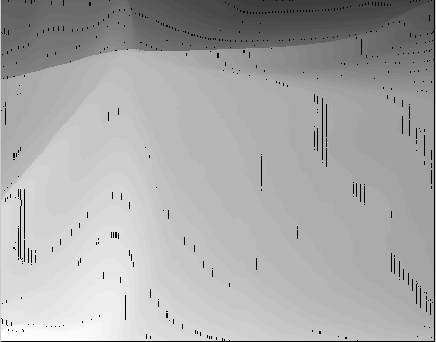
\includegraphics[scale=0.6]{disp3}
\end{figure}

\subsection{Part b}

Error rate for the map constructed using the closest pixel to camera: 0.4583 \newline
Error rate for the disparity map constructed using the pixel with smallest SAD cost: 0.4523

\begin{figure}[H]
  \caption{Disparity for view 3 using the pixels nearest to the camera}
  \centering
    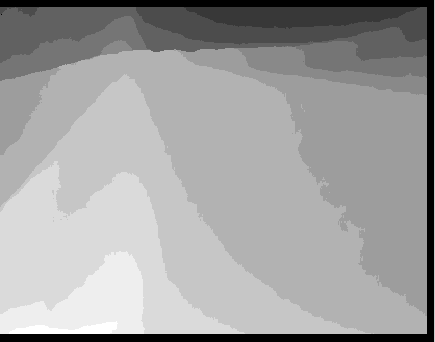
\includegraphics[scale=0.5]{dd1novo}
\end{figure}

\begin{figure}[H]
  \caption{Disparity for view 3 using the smallest SAD cost}
  \centering
    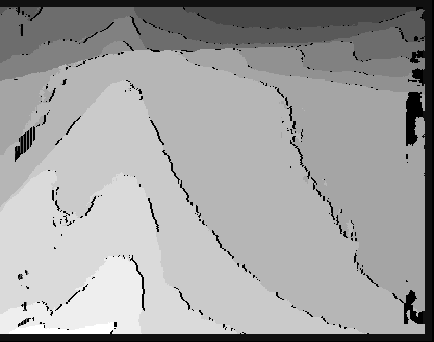
\includegraphics[scale=0.5]{dd2novo}
\end{figure}

\section{Matlab code}

\begin{lstlisting}[language=Matlab]

function cloud = get3dPoints(disparity, baseline, focal_length)
    z = baseline*focal_length./disparity;
    [x,y] = meshgrid(1:size(disparity,2), 1:size(disparity,1));
    x = baseline.*x./disparity;
    y = baseline.*y./disparity;
    cloud = [x(:) y(:) z(:)]';
end

function proj = projectInCamera(cloud, c, focal_length)
    proj = cloud - repmat(c,1,length(cloud));
    proj(1,:) = focal_length*proj(1,:)./proj(3,:);
    proj(2,:) = focal_length*proj(2,:)./proj(3,:);
end

function disparity = getDispFrom3d(cloud,baseline,focal_length, sz)
    disparity = zeros(sz);
    for i = 1:length(cloud)
        a = round(cloud(1,i));
        b = round(cloud(2,i));
        c = cloud(3,i);
        if a > 0 && b > 0 && ~isnan(a) && ~isnan(b) && ...
           a < size(disparity,2) && b < size(disparity,1) && c~=0
            disparity(b,a) = baseline*focal_length/c;
        end
    end
end

clc; clear all;

for i = 1:7
  data(:,:,i) = imread(['cloth3/view' num2str(i-1) '.pgm']); 
end

disp1 = imread('cloth3/disp1.pgm');
disp5 = imread('cloth3/disp5.pgm');
disp1 = double(disp1)./3;
disp5 = double(disp5)./3;

baseline = 40;
focal_length = 1247;
px = size(disp1,2)/2;
py = size(disp1,1)/2;
c1 = [0 0 0]';
c2 = [40 0 0]';
c3 = [80 0 0]';
c5 = [160 0 0]';

cloud1 = get3dPoints(disp1, 4*baseline, focal_length);
cloud31 = projectInCamera(cloud1, c3, focal_length);
disp31 = getDispFrom3d(cloud31, 4*baseline, focal_length, size(disp1));

cloud5 = get3dPoints(disp5, -4*baseline, focal_length);
cloud35 = projectInCamera(cloud5, c5-c3, focal_length);
disp35 = getDispFrom3d(cloud35, -4*baseline, focal_length, size(disp1));

disp3 = zeros(size(disp31));

for i = 1:size(disp31,1)
    for j = 1:size(disp31,2)
        disp3(i,j) = max([disp31(i,j) disp35(i,j)]);
    end
end

%%%%%%%%%%

% [d1,cost1] = stereoMatching(data(:,:,1), data(:,:,2), 1, 64, 0, 9);
% [d3,cost3] = stereoMatching(data(:,:,3), data(:,:,4), 1, 64, 0, 9);
% [d5,cost5] = stereoMatching(data(:,:,5), data(:,:,6), 1, 64, 0, 9);
% imwrite(uint8(d1), 'd1.pgm');
% imwrite(uint8(d3), 'd3.pgm');
% imwrite(uint8(d5), 'd5.pgm');
% imwrite(uint8(cost1), 'c1.pgm');
% imwrite(uint8(cost3), 'c3.pgm');
% imwrite(uint8(cost5), 'c5.pgm');

d1 = double(imread('d1.pgm'));
d3 = double(imread('d3.pgm'));
d5 = double(imread('d5.pgm'));
cost1 = double(imread('c1.pgm'));
cost3 = double(imread('c3.pgm'));
cost5 = double(imread('c5.pgm'));

% combining to generate disp 3

cloudd1 = get3dPoints(d1, baseline, focal_length);
cloudd31 = projectInCamera(cloudd1, c3, focal_length);
dispd31 = getDispFrom3d(cloudd31, baseline, focal_length, size(disp1));

cloudd5 = get3dPoints(d5, -baseline, focal_length);
cloudd35 = projectInCamera(cloudd5, c5-c3, focal_length);
dispd35 = getDispFrom3d(cloudd35, -baseline, focal_length, size(disp1));

% answers to disp3 using d1,d3,d5
dd1 = zeros(size(disp31));
dd2 = zeros(size(disp31));

for i = 1:size(disp1,1)
    for j = 1:size(disp1,2)
        dd1(i,j) = max([dispd31(i,j) dispd35(i,j) d3(i,j)]);
        
        [~,idx] = min([cost1(i,j) cost3(i,j) cost5(i,j)]);
        switch(idx)
            case 1, dd2(i,j) = dispd31(i,j);
            case 2, dd2(i,j) = d3(i,j);
            case 3, dd2(i,j) = dispd35(i,j);
        end
    end
end

% multiply by 4 so I can compare with 'disp3', which was generated using
% 4*baseline
dd1 = dd1.*4;
dd2 = dd2.*4;

miss1 = or(dd1 == 0, disp3 == 0);
miss2 = or(dd2 == 0, disp3 == 0);

total = size(dd1,1)*size(dd1,2);

err1 = abs((dd1(:) - disp3(:))) > 1;
err1 = sum(err1(~miss1))/(total - sum(sum(miss1)))

err2 = abs((dd2(:) - disp3(:))) > 1;
err2 = sum(err2(~miss2))/(total - sum(sum(miss2)))


\end{lstlisting}


\end{document}


